\chapter{A process prediction training Framework}\label{chap:training-framework}
During development of the models, we realized that there are highly divergent understandings regarding the batch construction for next-element predictions with sequences. We believe that these different understandings strongly impact the reproducibility of prediction approaches. Therefore we present here a framework that enables researchers to compare the different understandings and easily try out new model architectures. In doing so, we hope to contribute to Area 1 and 2 in \autoref{sec:intro:motivation}.

In this chapter, we show a selection of possible batch construction strategies in \autoref{sec:contrib:input-formatting} and the underlying technical reasons. Finally, we present the training framework in \autoref{sec:contrib:training-framework}.

\section{Contrasts among batching strategies}\label{sec:contrib:input-formatting}
We implemented the SP2 and PFS models as well as the comparison models using Python and the Keras neural networks API. While doing so, a wide range of recommended possibilities to train the models were noted in relevant publications and on online platforms such as StackOverflow.\\

Some recommend sliding window approaches, while others deem this against the concept of LSTM cells. Especially Klinkmüller et al. argue against it: "[...]the popular strategy of cutting traces to certain prefix lengths to learn prediction models for ongoing instances is prone to yield unreliable models"~\cite{klinkmuller2018reliablemonitoring}. Again others argue that padding and truncating sequences to the same length makes training faster and does not affect accuracy. Furthermore, the batch size represents an important hyper-parameter, and no guidelines how to sort traces into batches were found. We believe that the understanding of the merits of each batch construction strategy can be of general value to any application of sequence prediction.\\

Keras' implementation of LSTM is stateful \textit{during} a batch, and resets the cell state $C$ before the next batch~\cite{web:keras}. This is configurable, but for the sake of simplicity, it is advisable to keep related timesteps inside a single batch. Translated to traces, this means keeping a trace completely inside a batch. A Keras LSTM layer requires input data to be formatted in a three-dimensional array of fixed size for every batch. Each dimension has a defined meaning:

$$(n_{samples}, n_{timesteps}, n_{features})$$

Each sample contains a number of timesteps $n_{timesteps}$ containing a number of features $n_{features}$. $n_{features}$ is constant, as it represents the feature vector dimensions. For each sample, the Keras LSTM layer cells maintain a separate state, meaning that several traces can be trained on simultaneously~\cite{web:keras-lstm-state}. As the batches themselves need not to have the same dimensions, this definition opens up a range of possibilities to construct batches, four of which we highlight in the following paragraphs. To the best of our knowledge, these have not been compared in this context yet.\\

First and easiest, one trace can be trained per batch. This fulfills the requirement of constant dimensions, since only a single sample is used.

Second, \textit{some} traces can be trained inside a single batch. This is possible if all traces inside the batch have the same number of timesteps, i.e. have the same length. The number of samples and timesteps may vary between batches. A look at the trace length distribution in \autoref{fig:bpic2011-length-distribution} from BPIC11 reveals that grouped batching could bias the model toward the long tail of the distribution, as those traces are trained in batches of their own.

\begin{figure}[ht!]
    \centering
    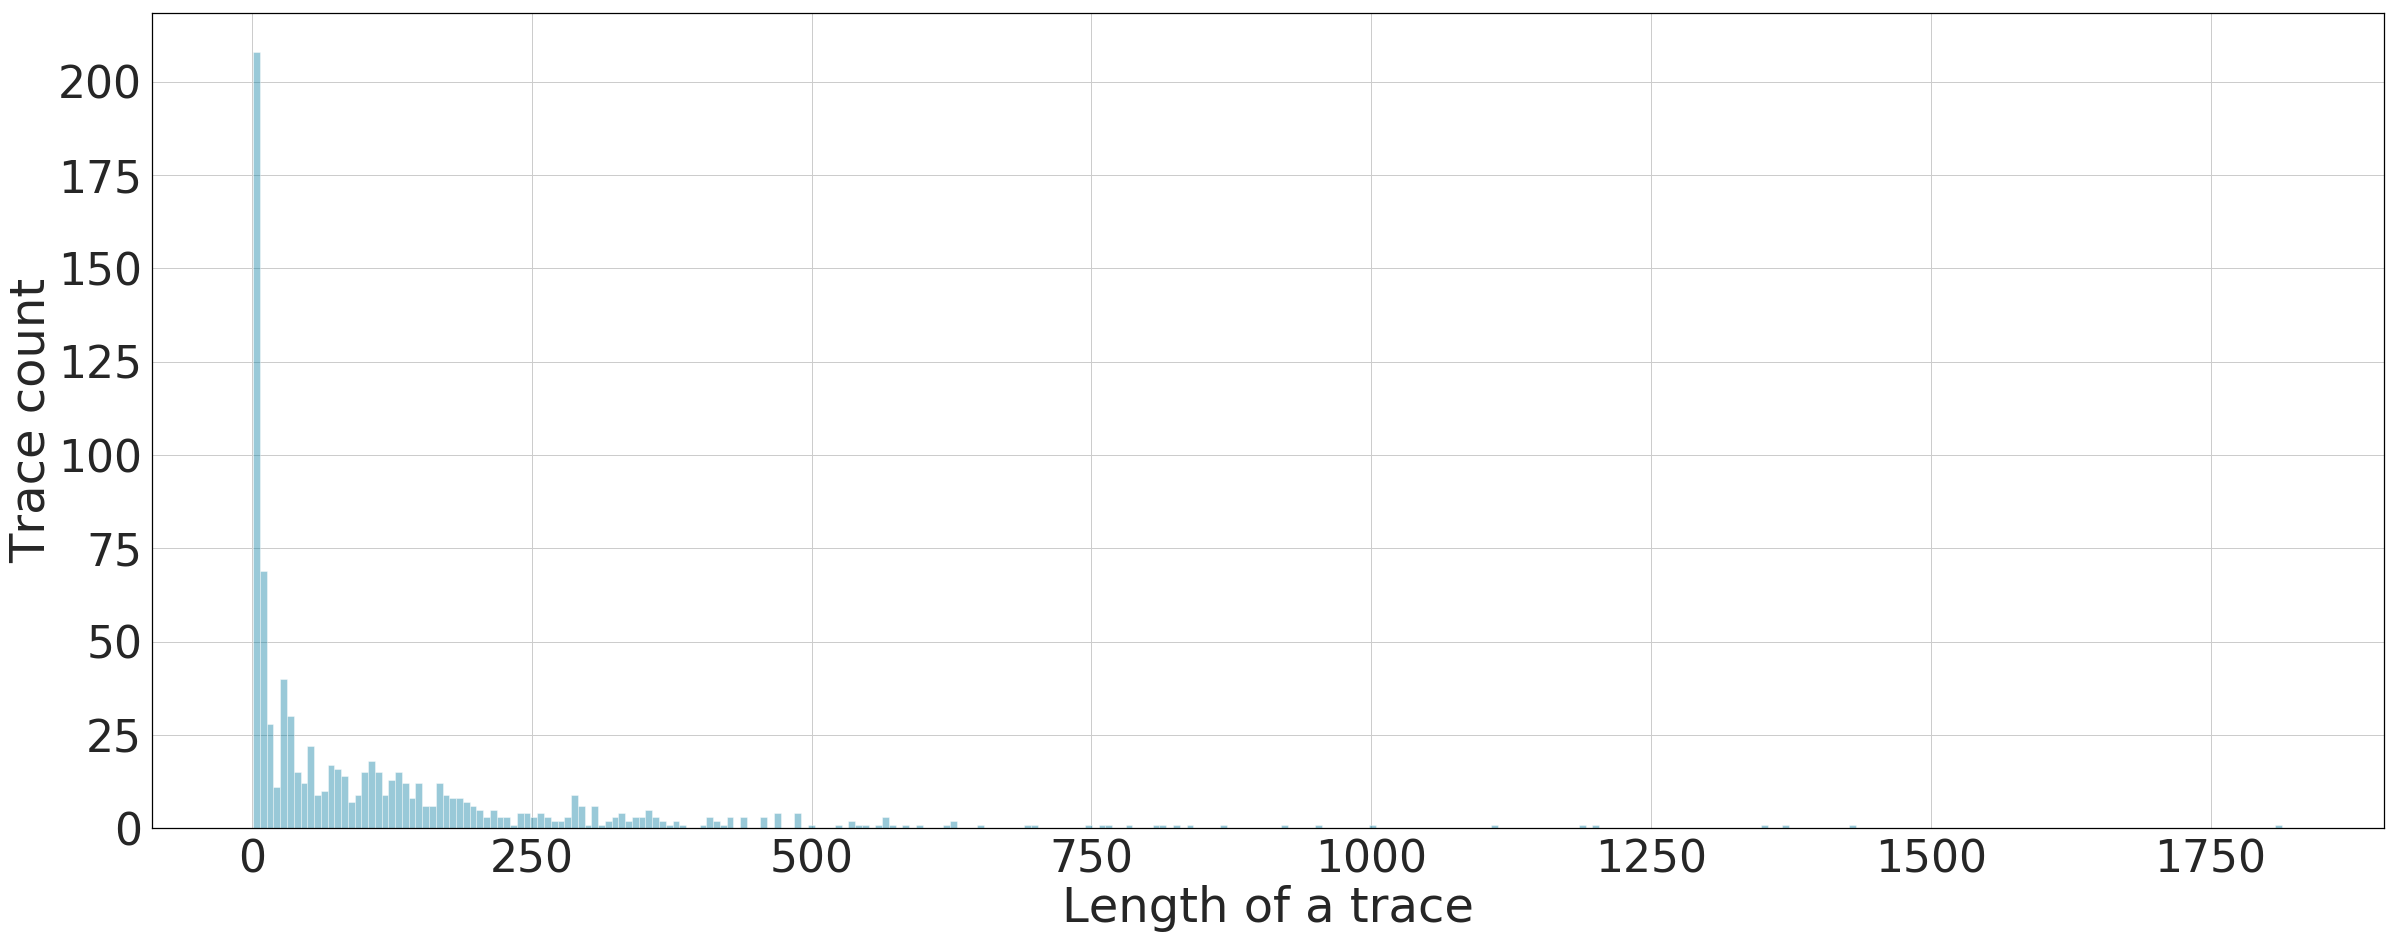
\includegraphics[width=.9\textwidth]{gfx/frequency-distribution.png}
    \caption{Distribution of trace lengths in BPIC11}
    \label{fig:bpic2011-length-distribution}
\end{figure}

Third, there is the possibility of padding the number of time-steps in a sequence to the same length and using a Masking layer to then filter out the padded values during training~\cite{web:keras}. The padding length is dictated by the maximum trace length and may incur a large memory overhead if it is a large outlier value like in BPIC11.

Fourth and finally, there is also the possibility to split the trace into samples by sliding a window along it. This results in $l-w+1$ samples for a trace of length $l$ and a window width $w$. Taking \autoref{tab:sliding-window} in \autoref{sec:background:feature-engineering} as an example, the window would be two timesteps wide. While this approach solves the problem of unequal sample lengths and facilitates batch construction, the model can only use a maximum of $w$ timesteps per sample for training and might lose potential long-term dependencies. As both Evermann et al.~\cite{evermann2016} and Schönig et al.~\cite{schoenig2018} use this format and it directly opposes the findings of Klinkmüller et al.~\cite{klinkmuller2018reliablemonitoring}, we investigate it. Furthermore, we are convinced that a windowed training data format misses out on LSTM potential.\\

The four batching strategies are labelled in the order of the preceding presentation for easier reference in the next chapter, where they are evaluated:
\begin{itemize}
\item\textbf{Individual}: One trace per batch
\item\textbf{Grouped}: Same-length traces in one batch
\item\textbf{Padded}: Padded-to-length traces
\item\textbf{Windowed}: Windowed samples, as used by Evermann and Schönig
\end{itemize}

\section{A next-event predictive model training framework}
\label{sec:contrib:training-framework}
We realize that making different process prediction approaches comparable is not only a technical but also a data-related challenge - no established benchmarking datasets for Predictive Process Monitoring exist yet.
To mitigate this situation, we designed a software framework that helped us compare the sixteen total model-batching-strategy combinations on a variety of datasets in an extensible way. We want to make this framework accessible to future researchers to facilitate model development, and sharing of implementations.\\

\begin{figure}
    \centering
    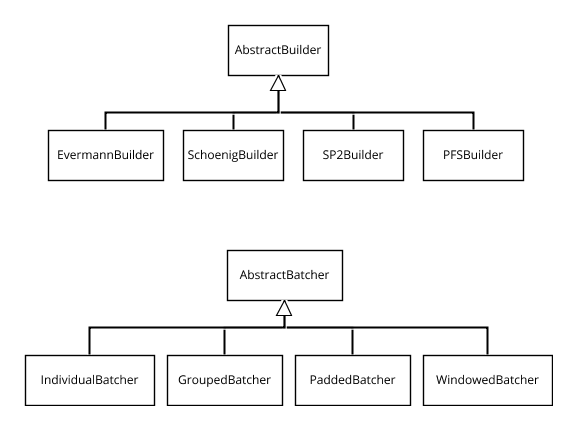
\includegraphics[width=\textwidth]{gfx/training-framework-classes.png}
    \caption[UML diagram of the framework classes]{Unified Modeling Language (UML) diagram of the abstract base class inheritance structure of Builders and Batchers}
    \label{fig:trainig-framework-classes}
\end{figure}

The proposed framework provides a simple training frontend, and integrates two concepts: Builders and Batchers. As \autoref{fig:trainig-framework-classes} shows, the two concepts are introduced as abstract base classes from which the actual model and batching strategy implementations are derived.\\

\noindent\textbf{Builders} construct Keras models and also define the structure of the training and test data. This is important as models may not only have one input layer, but two or more. These pre-formatted data sets are not structured into batches yet. One such Builder is implemented for every model type by inheriting from the abstract base class \verb=AbstractBuilder=.\\

\noindent\textbf{Batchers} take the pre-formatted data sets and structure them into batches. For each batching strategy, a class inherits from the abstract base class \verb=AbstractBuilder=.\\

\noindent The \verb=model_runner= frontend ties these two concepts together with training logic and provides a basic command-line interface as \autoref{fig:framework-frontend} shows. It allows for flexibly training a model with a specific Builder and a specific Batcher. It also permits placing the training process on a specific GPU, and defining the output directory for the model and performance measurement files. The training algorithm also implements early stopping, of which the thresholds can be configured via a configuration file.\\

%The inheritance structure allows all classes to implement the same interface, which make the interaction in \autoref{fig:} possible. This exchange enables the flexibility that this framework provides.\\

With the help of this framework, future researchers only need to subclass \verb=AbstractBuilder=, and can directly evaluate the model performance on any given dataset without having to implement the whole training environment. By simply sharing their Builder and Batcher implementations, it will be much easier for other researchers to reproduce findings. The framework and detailed documentation is hosted under \href{https://github.com/flxw/nitro4ppm}{flxw/nitro4ppm}

\begin{figure}
\centering
\begin{verbatim}
usage: model_runner.py [-h] [--gpu GPU]
                       [--output OUTPUT]
                       {evermann,schoenig,sp2,pfs}
                       {padded,grouped,individual,windowed}
                       datapath

The network training framework script for Felix Wolff's master's thesis!

positional arguments:
  {evermann,schoenig,sp2,pfs}
                        Which type of model to train.
  {padded,grouped,individual,windowed}
                        Which mode to use for feeding
                        the data into the model.
  datapath              Path of dataset to use for training.

optional arguments:
  -h, --help            show this help message and exit
  --gpu GPU             CUDA ID of which GPU the model
                        should be placed on to
  --output OUTPUT       Target directory to put model
                        and training statistics
\end{verbatim}
\caption[CLI frontend for the framework]{The \texttt{model\_runner} command-line frontend for the training framework}
\label{fig:framework-frontend}
\end{figure}
